% !TeX root = ../main.tex
% !TEX root = ../main.tex
% -*- root: ../main.tex -*-
% -*- program: pdflatex -*-
\chapter{人工神经网络}
\section{神经元模型}
人类的大脑思维能力是人类智能的重要体现。大脑的神经网络系统中,神经元(neuron)是处理信息的基本单元。它由四部分组成:细胞体,树突,轴突和突触。树突接受外来信息,并传递给细胞体,是神经元细胞的输入通道;细胞体主要作用为接受并处理信息,是神经元细胞的新陈代谢中心;轴突向外传递信号,是神经元细胞的输出通道;突触为神经元末梢与另一神经元的细胞体或树突的接触,是神经元细胞的输入输出接口。图~\ref{fig:neuron}~为神经元结构的示意图。神经元有兴奋和抑制两种状态,其工作原理为:处于抑制状态的神经元,树突接受外来脉冲信号传递给细胞体,如果有多个树突传递则以代数和的方式叠加;如果输入的脉冲信号超出某个阈值,则神经元进入兴奋状态,并通过轴突向其它神经元传递信号。
\begin{figure}[!htb]
  \centering
  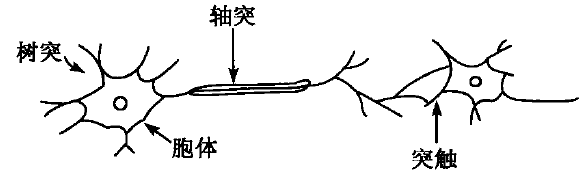
\includegraphics[width=10cm]{chap2/neuron.png}
  \caption{神经元结构示意图}
  \label{fig:neuron}
\end{figure}

人工神经元是一种模仿生物神经元信息传递方式的数学模型,其结构示意图如图\ref{fig:MP}~所示。
\begin{figure}[!htb]
  \centering
  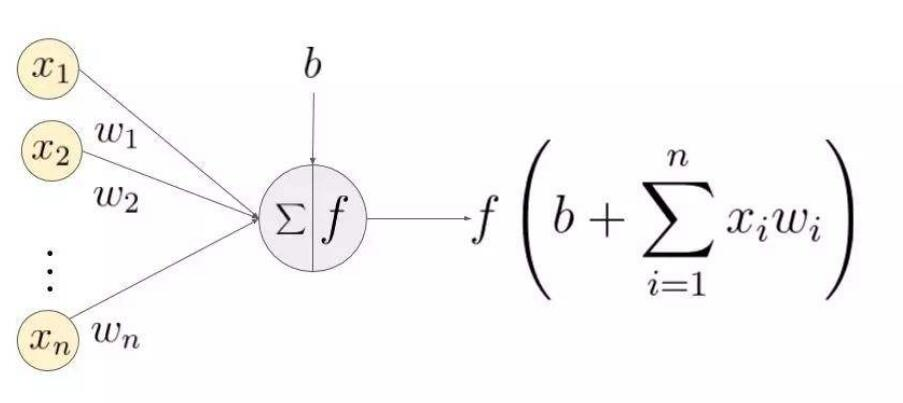
\includegraphics[width=10cm]{chap2/MP.jpg}
  \caption{人工神经元}
  \label{fig:MP}
\end{figure}

图中,$x_{1}, x_{2}, …, x_{n}$~为外界的输入信号,相当于神经元的树突;$w_{1}, w_{2}, …, w_{n}$~为输入信号的权重(weight),相当于神经元中突触的连接强度;$\sum$表示对n个输入信号的累加,f为对累加信号的响应,成为激活函数,类似于神经元的细胞体;b为偏置项(bias),类似于神经元的激活阈值。神经元的输入可表示为:
$$input = \sum_{i=1}^{n}w_{i}x_{i} +b = \sum_{i=0}^{n}w_{i}x_{i}  (x_{0} = b, w_{0} = 1)$$
输出为:
$$output = f(input)$$
常见的激活函数有:

(1).线性函数
$$f(x) = x$$

(2).符号函数
$$f(x) = sgn(x) = \left\{
\begin{aligned}
1, x \geq 0 \\
-1, x < 0
\end{aligned}
\right.
$$

(3).饱和函数
$$f(x) = \left\{
\begin{aligned}
1, &x \geq \frac{1}{k} \\
kx, &-\frac{1}{k} \leq x < \frac{1}{k}\\
-1, &x < -\frac{1}{k}
\end{aligned}
\right.
$$

(4).双曲正切函数
$$f(x) = th(x) = \frac{1-e^{-x}}{1+e^{-x}} = \frac{2}{1+e^{-x}} -1$$

(5).阶跃函数
$$f(x) = sgn(x) = \left\{
\begin{aligned}
1, x \geq 0 \\
0, x < 0
\end{aligned}
\right.
$$

(6).Sigmoid函数
$$f(x) = \frac{1}{1+e^{-x}}$$

(7).Relu函数
$$f(x) = max{0,x}$$

\section{神经网络基本结构}
把许多人工神经元按照特定的层次结构连接起来,就得到神经网络。本文采用全连接型神经网络(Fully Connected neural network),其连接方式如图\ref{fig:neural_network}~所示。全连接神经网络每一层与下一层神经元互相连接,同层之间的神经元不连接,包含输入层( input layer ),隐层( hidden layer )和输出层( output layer )。输入层接受输入信号,并将其传递给隐层;隐层接受上一层传递的信号,将其通过激活函数处理后传递给下一层;输出层输出网络的分类结果。
\begin{figure}[!htb]
  \centering
  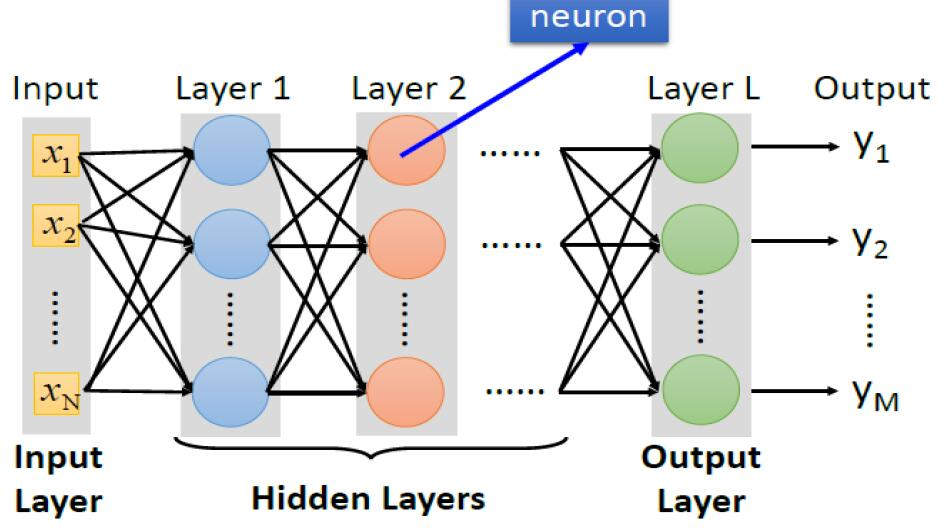
\includegraphics[width=10cm]{chap2/neural_network.jpg}
  \caption{全连接神经网络示意图}
  \label{fig:neural_network}
\end{figure}
\section{前向传播与反向传播}
神经网络更新神经元的方式为根据输入层的值以及每个值的权重更新第一层的输出值,再根据第一层的输出值及每个输出值的权重更新第二层的输出值,依次类推直至更新输出层的输出值,此过程为正向传播过程。其计算公式为:
$$z_{j} = f(\sum_{i} w_{ji}z_{j-1})$$
其中$z_{j}$表示网络中第j层神经元的输出值,$w_{ji}$表示j-1层中第i个神经元同第j层神经元的连接权重。通过前向传播获得输出层的之后,通过输出层与真实值比较,得到损失函数L。损失函数有多重形式,本文采用交叉熵损失函数,其计算方式为:
$$L = -\frac{1}{m}\sum^{m}_{i=1}[ y^{i}log\hat{y}^{i}+(1-y^{i})log(1-\hat{y}^{i}) ]$$
其中,$y^{i}$表示第i类的真实值(0或1),$\hat{y}^{i}$表示第i类神经网络在输出层的输出值。

通过损失你函数从后往前算出隐含层更单元的梯度,并以此修正各层之间的权重,此过程为反向传播过程。具体过程为:\\
输出层权重梯度:
$$\Delta{w^{L}} = \frac{\partial{L}}{\partial{\hat{y}}}*\frac{\partial{\hat{y}}}{\partial{w^{L}}}$$
输出层权重调整:
$$w^{L} = w^{L} + \Delta{w^{L}}$$
隐层权重梯度:
$$\frac{\partial{L}}{\partial{z^{l}}} = \frac{\partial{L}}{\partial{z^{l+1}}}*\frac{\partial{z^{l+1}}}{\partial{z^{l}}}$$
$$\Delta{w^{l}} = \frac{\partial{L}}{\partial{z^{l}}}*\frac{\partial{z^{l}}}{\partial{w^{l}}} = \frac{\partial{L}}{\partial{z^{l+1}}}*\frac{\partial{z^{l+1}}}{\partial{z^{l}}}*\frac{\partial{z^{l}}}{\partial{w^{l}}}$$
隐层权重调整:
$$w^{l} = w^{l} + \Delta{w^{l}}$$

%记得醒来时增加流程内容








(1).神经网络:
准确率:
0.791
参数:
hidden layers 5:
Dropout:0.3 for the layer 4 and layer5 
L2 regularizer:0. 00003
Epochs:50
running time:1950.1
Val accuracy:0.791
